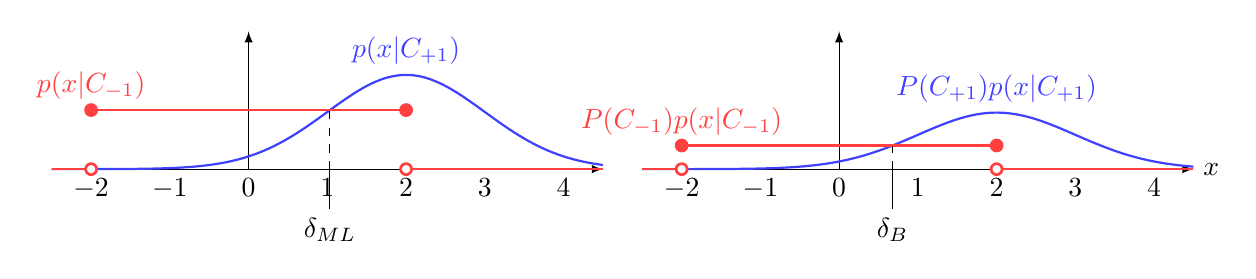
\begin{tikzpicture}[> = latex, domain=-2.5:4.5, samples=100]
    \def\r{1.75 * 0.05}
    \def\yScale{3}
    % Distributions before priors: Maximum-Likelihood estimator
    % Axis
    \draw [->] (-2.5, 0) -- (4.5, 0);
    \draw [->] (0, 0) -- (0, 1.75);
    \foreach \x in {-2, -1, 0, 1, 2, 3, 4}{
        \draw (\x, 0) node [below] {$\x$};
    }
    % p(x|C+1)
    \draw [thick, blue!75] 
        plot (\x, {\yScale * 0.39894 * exp(-0.5 * (\x-2) * (\x-2))})
        (2, \yScale * 0.39894) node [above] {$p(x|C_{+1})$};
    % p(x|C-1)
    \def\deltaML{1.033} % 
    \draw [thick, red!75] 
        (-2, \yScale * 1/4) node [above] {$p(x|C_{-1})$} --++ (4, 0)
        (2, 0) -- (4.5, 0)
        (-2, 0) -- (-2.5, 0)
    ;
    \fill [red!75]
        (-2, \yScale * 1/4) circle (\r)
        (2, \yScale * 1/4) circle (\r)
        (-2, 0) circle (\r)
        (2, 0) circle (\r)
    ;
    \fill [white]
        (-2, 0) circle (\r-1.75 * 0.02)
        (2, 0) circle (\r-1.75 * 0.02)
    ;
    \draw (\deltaML, 0) --++ (0, -0.5) node [below] {$\delta_\text{ML}$};
    \draw [dashed] (\deltaML, 0) --++ (0, \yScale * 1/4);

    % Distributions after priors: Bayes estimator (optimal)
    \def\deltaB{0.67877} % 
    \def\priorOne{0.6}
    \def\priorMinusOne{0.4}
    \begin{scope}[shift={(7.5, 0)}]
        % Axis
        \draw [->] (-2.5, 0) -- (4.5, 0) node [right] {$x$};
        \draw [->] (0, 0) -- (0, 1.75);
        \foreach \x in {-2, -1, 0, 1, 2, 3, 4}{
            \draw (\x, 0) node [below] {$\x$};
        }
        % p(x|C+1)
        \draw [thick, blue!75] 
            plot (\x, {\yScale * \priorOne * 0.39894 * exp(-0.5 * (\x-2) * (\x-2))})
            (2, \yScale * \priorOne * 0.39894) node [above] {$P(C_{+1}) p(x|C_{+1})$};
        % p(x|C-1)
        \draw [thick, red!75] 
            (-2, \yScale * \priorMinusOne * 1/4) node [above] {$P(C_{-1}) p(x|C_{-1})$} --++ (4, 0)
            (2, 0) -- (4.5, 0)
            (-2, 0) -- (-2.5, 0)
        ;
        \fill [red!75]
            (-2, \yScale * \priorMinusOne * 1/4) circle (\r)
            (2, \yScale * \priorMinusOne * 1/4) circle (\r)
            (-2, 0) circle (\r)
            (2, 0) circle (\r)
        ;
        \fill [white]
            (-2, 0) circle (\r-1.75 * 0.02)
            (2, 0) circle (\r-1.75 * 0.02)
        ;
        \draw (\deltaB, 0) --++ (0, -0.5) node [below] {$\delta_\text{B}$};
        \draw [dashed] (\deltaB, 0) --++ (0, \yScale * \priorMinusOne * 1/4);
    \end{scope}
\end{tikzpicture}